
\section{Low-rank Matrices}

In practice, most matrices are large, so storing each element is not efficient, or even possible for some physical setups. If $A \in \mathbb{C}^{n\times m}$ has a rank \textit{k} such that $k \leq m$ and $k(n+m) < n*m$ (\textit{A} is low-rank), \textit{A} can be written in outer product form, as a product between the matrices $U \in \mathbb{C}^{n\times k} $ and $V \in \mathbb{C}^{m\times k}$, which can be seen in \ref{eq::outer_product}, where $u_{i}, v_{i}$ are the column vectors of \textit{U} and \textit{V}.

\begin{equation}\label{eq::outer_product}
    A = UV^{H} = \sum_{i=1} ^{k} u_{i} v_{i} ^{*}
\end{equation}


Therefore, storing $k(n+m)$ elements to write $A$, and not $n\times m$. A matrix \textit{A} that can be represented as \ref{eq::outer_product} is an element of $\mathbb{C}^{n\times m}_{k}$.

The representation in \ref{eq::outer_product} also facilitates other operations with $A$, like matrix-vector products $Ab$ that are always present in methods like GMRES \cite{bebendorf2008hierarchical} and different kinds of norms, like $\norm{A}_{F}, \norm{A}_{2}$ \cite{bebendorf2008hierarchical}.

However, even full rank matrices can be approximated by matrices with lower rank. A theorem \cite{bebendorf2008hierarchical} establishes that the closest matrix from $\mathbb{C}^{n\times m}_{k}$ of a matrix from $\mathbb{C}^{n\times m}$ can be obtained from the SVD $A = U \Sigma V^{H}$, where $\Sigma$ contains the singular valuers $\sigma_{1} \geq \sigma_{2} \dots \sigma_{m} \geq 0$ and $U,V$ are unitary.

If $ A_{k} $ is the approximation obtained after taking the first k elements of $\Sigma$ (creating the matrix $ \Sigma_{k} $), the error between $ A $ and $ A_{k} $ is \ref{eq:error_lowrank}.

\begin{equation}\label{eq:error_lowrank}
    \norm{A-A_{k}} = \norm{U\Sigma V^{H} - U^{'} \Sigma_{k} V^{' H}} = \norm{\Sigma - \Sigma_{k}}
\end{equation}

If the spectral norm, $\norm{.}_{2} $ is used instead, the error in \ref{eq:error_lowrank} is given by $\sigma_{k+1}$. For Frobenius's norm, $\norm{.}_{F}$, the error becomes $\sqrt{\sum^{n}_{l=k+1} \sigma^{2}_{l}}$.

If a problem involves a large matrix that is not low-rank, it can have sub-blocks that can be approximated by matrices of this kind. Blocks that appear after the discretization of elliptic operators also have the possibility of being approximated by matrices that decay exponentially with k, $S_{k}$, as in \ref{eq:exp_matrix}.

\begin{equation}\label{eq:exp_matrix}
    \norm{A-S_{k}}_{2} < q^{k}\norm{A}_{2}
\end{equation}


% That way the rank, and precision are related logarithmically, and the rank required by a certain $\epsilon$ is \ref{eq:exp_error}.

% \begin{equation}\label{eq:exp_error}
%     k(\epsilon) = \min\{ k \in \mathbb{N} : \sigma_{k+1} < \epsilon\sigma_{1}\}
% \end{equation}

\section{ACA Method(Adaptative Cross Approximation)}

As shown in the last section, the SVD method gives us an approximation of $A$ given a certain $\epsilon$, through the relation in \ref{eq:error_lowrank}. Nevertheless, this is an expensive method. Not only having a large complexity, but also requiring knowledge of every element of the block going to be compressed.

The algorithm for the method is in \ref{alg:aca_method}, where $a_{ij}$ are the elements of a matrix $A \in \mathbb{R}^{n\times m}$ and $\kappa$ at the stopping criterion is the cluster parameter for a certain admissibility condition(discussed in the next section). The main objective is to approximate $A$ as $A=S_{k} + R_{k}$, $S_{k} = \sum_{l=1}^{k} u_{l}v_{l}^{t}$ and $R_{k}$ is the residual.



\begin{algorithm}
    \caption{ACA Method}\label{alg:aca_method}
    \begin{algorithmic}[1]
        \State $k=1$ et $\mathbf{Z} = \emptyset $
        \Repeat
        \State Find $i_{k}$
        \State $\hat{v}_{k} = a_{i_{k},1:m} $
        \For{$l=1,\dots , k-1$}
        \State $\hat{v}_{k} = \hat{v}_{k} - (u_{l})_{i_{k}}v_{l} $
        \EndFor
        \State $Z = Z \bigcup \{ i_{k} \} $

        \If{$\hat{v}_{k}$ does not vanish}
        \State $j_{k} = argmax_{j=1, \dots, m}|(\hat{v}_{k})_{j}|$
        \State $v_{k} = (\hat{v}_{k})^{-1}_{j_{k}} \hat{v}_{k}$
        \State $u_{k}=a_{1:n,j_{k}}$

        \For{$l=1,\dots,k-1$}
        \State $u_{k}=u_{k} - (v_{l})_{j_{k}}u_{l}$
        \EndFor
        \State $k=k+1$

        \EndIf


        \Until{$\norm{u_{k}}_{2}\norm{v_{k}}_{2} \leq \frac{\epsilon(1-\kappa )}{1+\epsilon}\norm{S_{k}}_{F}$}

    \end{algorithmic}
\end{algorithm}

And then, for the Frobenius Norm, it can be show \cite{trefethen1998numerical}(Section 3.4.1) that:

\begin{equation}\label{eq:stop_ACA}
    \frac{\norm{A - S_{k}}_{F}}{\norm{A}_{F}} = \epsilon
\end{equation}

\section{Hierarchical Matrices}

Going a little more in depth about the use of low-rank approximations in larger matrices that are not really low-rank themselves, we present the concepts of \textit{partition} and \textit{admissibility}.

As mentioned in the first section of this chapter, even if  $A \in \mathbb{C}^{m \times n} $ cannot be entirely approximated by a low-rank matrix, in the context we work with it can still be approximated in its sub-blocks. More specifically, in the sub-blocks of a proper partition $P$ of the matrix indices.

Using $I = {1,2, \dots, m}$ and $J={1,2, \dots, n}$, a subset $P$ from the set of subsets of $I \times J$ is called a partition if:

\begin{equation}\label{eq:union_partition}
    I \times J = \bigcup_{b \in P} b
\end{equation}

Where if $b_{1} \cap b_{2} \neq \varnothing $ then $b_{1} = b_{2}$.

From here on out we also use the notation $A_{b}$ or $A_{ts}$ for the restriction of a matrix $A$ to the indices in $b= t \times s$ where $b \in P$, $t \in I$ and $s \in J$.

The many algorithms that compress a given matrix have to make sure $A_{b}$ will either be approximated by a low-rank block or is very small(making sure storing its elements will not be expensive). The number of blocks compressed in a matrix also should not be large.

The problem of knowing whether a block can be compressed comes from the abstract concept of \textit{admissibility}, usually relying on the specific problem we solve. Nevertheless, \textit{admissibility conditions} can be established that each one of the compressed blocks need to satisfy:

\begin{itemize}
    \item If \textit{b} is admissible, then its singular values decay exponentially;
    \item the admissibility condition for a block $t \times s$ can be verified with $\mathcal{O}(|t| + |s|)$;
    \item if $b$ is admissible, then $b^{'} \in b$ also is.
\end{itemize}

A partition $P$ is said admissible if every one of its blocks are either admissible or small, i.e., $|t|, |s|$, with $t \in I, s \in J$, satisfy $\min\{|t|,|s| \} \leq n_{min}$ for a given $n_{min} \in \mathbb{N}$.

Although the partition P has been mentioned multiple times throughout the text, we have not disclosed how such partition could be made.

It's obvious searching the entire set of partitions $P$ of $I \times J$ is unfeasible, so the partitions are usually  recursive subdivisions of both $I$ and $J$. And it's shown such partitions can lead to linear complexity \cite{bebendorf2008hierarchical}.

The result of the recursive division of a set results in a hierarchy of partitions that can be represented as a \textit{cluster tree}.

We denote this cluster tree associated with the subdivisions of $I$ as $T_{I} = (V,E)$, with vertices $t \in V$ and edges $E$. The set $S(t)={t^{'} \in V : (t,t^{'})\in E}$ is the set of sons of $t$. By $\mathfrak{L}(T_{I})$, we denote the set of leaves of $T_{I}$:

\begin{equation}
    \mathfrak{L}(T_{I}) = \{ t : S(t) = \emptyset \}
\end{equation}

The conditions such tree $T_{I}$ must follow are:

\begin{enumerate}
    \item $I$ is the root of $T_{I}$;
    \item $\varnothing \neq t = \bigcup_{t^{'} \in S(t)} t^{'} $ for all $t \in V \setminus   \mathfrak{L}(T_{I}) $;
    \item the degree $\deg t := |S(t)| \geq 2$ of each vertex $t \in V \setminus \mathfrak{L}(T_{I})$ is bounded from below.
\end{enumerate}

As an illustration of the concept, we draw the balanced binary cluster tree of the set $I=\{1,2,3,4,5,6,7,8\}$ in \autoref{fig:cluster_tree}.

\begin{figure}[!h]

    \centering
    \begin{tikzpicture}\label{tree:cluster}
        \tikzstyle{level 1}=[sibling distance=30mm]
        \tikzstyle{level 2}=[sibling distance=10mm]
        \tikzstyle{level 3}=[sibling distance=5mm]
        \tikzstyle{level 4}=[sibling distance=5mm]
        \node(root){I = \{1,2,3,4,5,6,7,8\}}
        child
            {
                node{\{1,2,3,4\}}
                child
                    {
                        node{\{1,2\}}
                        child{node{\{1\}}}
                        child{node{\{2\}}}
                    }
                child
                    {
                        node{\{3,4\}}
                        child{node{\{3\}}}
                        child{node{\{4\}}}
                    }
            }
        child
            {
                node(level1){\{5,6,7,8\}}
                child
                    {
                        node{\{5,6\}}
                        child{node{\{5\}}}
                        child{node{\{6\}}}
                    }
                child
                    {
                        node(level2){\{7,8\}}
                        child{node{\{7\}}}
                        child{node(level3){\{8\}}}
                    }
            };

        \coordinate (right) at ($(current bounding box.east) + (1,0)$);
        \node at (root -| right) {Level 0};
        \node at (level1 -| right) {Level 1};
        \node at (level2 -| right) {Level 2};
        \node at (level3 -| right){Level 3};
    \end{tikzpicture}

    \caption{Example tree of the set $I=\{1,2,3,4,5,6,7,8\}$.}
    \label{fig:cluster_tree}
\end{figure}

For clarification, we also show how a vector $x \in \mathbb{R}^{I}$ can be structured into a \textit{block vector} with the use of a cluster tree, using a partition $P=\{t_{1}, t_{2}, t_{3}, t_{4}\}$ of $I$, with the same definition as in \ref{eq:union_partition}, i.e., $I = \bigcup_{t \in P} t$.

With $t_{1} = \{1\}, t_{2} = \{2\}, t_{3}=\{3,4\}$ and $t_{4}=\{5,6,7,8\}$ we have the following block structure for $x=\{x_{1},x_{2},x_{3},x_{4},x_{5},x_{6},x_{7},x_{8}\}$:

\begin{equation}
    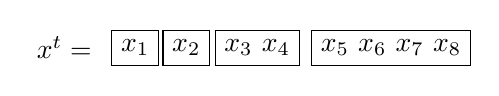
\begin{tikzpicture}[
            grow=right,
            level 1/.style={level distance = 9mm},
            level 2/.style={level distance = 6.5mm},
            level 3/.style={level distance = 9mm},
            level 4/.style={level distance = 17mm}
        ]
        \node {$x^{t} = $}
        child{node[rectangle,draw]{$x_{1}$} edge from parent[draw=none]
        child{node[rectangle,draw]{$x_{2}$}edge from parent[draw=none]
        child{
        node[rectangle,draw]{$x_{3}$ $x_{4}$} edge from parent[draw=none]
        child{
        node[rectangle,draw]{$x_{5}$ $x_{6}$ $x_{7}$ $x_{8}$} edge from parent[draw=none]
        }
        }
        }
        }
        ;
    \end{tikzpicture}
\end{equation}

That would be represented by the subtree $T_{I} ^{'} \subset T_{I}$ with same root $I$:

\begin{figure}[!h]

    \centering
    \begin{tikzpicture}\label{tree:cluster}
        \tikzstyle{level 1}=[sibling distance=30mm]
        \tikzstyle{level 2}=[sibling distance=10mm]
        \tikzstyle{level 3}=[sibling distance=5mm]
        \tikzstyle{level 4}=[sibling distance=5mm]
        \node(root){I = \{1,2,3,4,5,6,7,8\}}
        child
            {
                node{\{1,2,3,4\}}
                child
                    {
                        node{\{1,2\}}
                        child{node{\{1\}}}
                        child{node(level3){\{2\}}}
                    }
                child
                    {
                        node(level2){\{3,4\}}
                    }
            }
        child
            {
                node(level1){\{5,6,7,8\}}       
            };

        \coordinate (right) at ($(current bounding box.east) + (1,0)$);
        \node at (root -| right) {Level 0};
        \node at (level1 -| right) {Level 1};
        \node at (level2 -| right) {Level 2};
        \node at (level3 -| right){Level 3};
    \end{tikzpicture}

    \caption{test.}
    \label{fig:xcluster_tree}
\end{figure}

Where its leaves, as shown above, coincide with the partition $P$ of $x$ in blocks. It can be stated \cite{hackbusch2015hierarchical} that any partition of $I$ can be described as a leaf set of a tree $T^{'}_{I} \in T_{I}$, just as any subtree $T_{I}^{'}$ can be associated with a partition $P \in I$.
%FIXME: fix the trees structure and distance between simblings, its weird...

To make a hierarchical structure for the \textit{blocks} of a matrix, we extend the notion of this partition tree to $I \times J$, which contains the indices of said matrix. Thus, we have in each of its leaves, the set $\mathfrak{L}(T_{I \times J})$, one admissible block of the partition.

This cluster tree $T_{I \times J}$ for $I \times J$ is called a \textit{block cluster tree}.


The set of hierarchical matrices in $\mathbf{T}_{I \times J}$ with rank k for each block $A_{b}$ is defined in \ref{eq:matrix_hier}.

\begin{equation}\label{eq:matrix_hier}
    \mathfrak{H}(\mathbf{T}_{I \times J},k) = \left\{  A\in \mathbb{C}^{I\times J} : rankA_{b} \leq k, \forall b \in P \right\}
\end{equation}

%FIXME: HMatrix figure right here, make things more visual


In practice, \ref{alg:aca_method} works with $\epsilon$ given by the user during the assembling of the Hierarchical Matrix, and the compression acts in each of the admissible blocks that will then be represented as low rank matrices, shown in \ref{eq::outer_product}. We also store each one of the residuals obtained in the outer loop of \ref{alg:aca_method}.

After giving a tolerance $\nu  \leq \epsilon$ for an inexact product, the algorithm, for each admissible block of the cluster tree, uses the right amount of columns $k^{'}$ of the outer product representation of the block as to reach the desired tolerance. The number of columns can be inferred by using the list of residuals of the ACA Method. A brief explanation can be found in \ref{alg:inexact_product}.

\begin{algorithm}
    \caption{Inexact Product algorithm.}\label{alg:inexact_product}
    \begin{algorithmic}[1]
        \State Be $\nu \in \mathbb{R}$, $b \in P$ the tolerance for the product,  $A_{b}= \sum_{i=1}^{k}u_{i}v_{i}^{*}$ a restriction of $A$ to one of its admissible blocks and $r \in \mathbb{R^{k}}$ a vector with the residuals obtained in each step of the ACA.
        \For{$k^{'} \in \{1, \dots, k \}$}
        \State $\alpha \leftarrow r_{k^{'}}$
        \If{$\alpha \leq \nu$}
        \State $\tilde{A_{b}}=\sum_{i=1}^{k^{'}}u_{i}v_{i}^{*}$
        \EndIf
        \EndFor

    \end{algorithmic}
\end{algorithm}

Where, if no value smaller than $\nu$ is found, we use all $k$ columns of each block to execute the product.

So, the different perturbations $E_{k}$ used in \ref{eq:new_projection} are the matrices that, when added to $A$, leave each admissible block with the right amount $k^{'}$ of columns in \ref{eq::outer_product}, so the product can be approximated by the tolerance $\nu$. Calling the approximation of each block $A_{b}$ as $\tilde{A_{b}}$, we have \ref{eq:inexact_productblock}.

\begin{equation}\label{eq:inexact_productblock}
    \frac{\norm{A_{b}q - \tilde{A_{b}}q }}{\norm{A_{b}q}} \leq \nu, \hspace{0.3in} \tilde{A_{b}} = \sum_{i=1} ^{k^{'}} u_{i} v_{i} ^{*}
\end{equation}


And then, since the Frobenius norm of the hierarchical matrix is \cite{hackbusch2015hierarchical}(Section 3.5.1):

\begin{equation}
    \norm{E_{k}}_{F}= \norm{\mathcal{A}_{k} - A} = \sqrt{\sum_{b \in P} \norm{A_{b} - \tilde{A_{b}}}_{F}^{2} }
\end{equation}

%this line is completely wrong, ill change it afterwards
But from the ACA Method \ref{eq:stop_ACA}, we know the method stops as to make each block's successive approximation inferior to previous one by a factor of $\epsilon$, then:

\begin{equation}
    \norm{E_{k}}_{F} = \sqrt{\sum_{b \in P} \norm{A_{b} - \tilde{A_{b}}}_{F}^{2} } \leq \sqrt{\sum_{b\in P}\epsilon^{2}\norm{A_{b}}_{F}^{2}} = \epsilon \sqrt{\sum_{b \in P}\norm{A_{b}}_{F}^{2}}
    \leq \epsilon \norm{A}_{F}
\end{equation}


%FIXME: Fix this, ||Ek|| != e_{k} ||Ek|| prop e_{k} ||A||
% So, with the use of the relative errors and the Frobenius norm, $\norm{E_{i}}$ appearing in the bounds of section 2.2 can be exchanged by $\epsilon_{i}$, the tolerance used for that specific approximation in the inexact products.

With this result, we can then substitute $\norm{E_{k}}$ appearing in the upper bounds of \autoref{chap:gmres}, using the fact that $E_{k}\propto \epsilon_{k} \norm{A}$, where $\epsilon_{k}$ is the tolerance used in the k-th inexact matrix-vector product.

%FIXME: write sigma = ||(\tilde{B} b) - B b|| relate it to the block approximations


